
\documentclass[11pt,a4paper]{article}

\usepackage[T1]{fontenc}
\usepackage[utf8]{inputenc}
\usepackage[dutch]{babel}
\usepackage{lmodern}
\usepackage{microtype}
\usepackage[a4paper,margin=2.0cm]{geometry}
\usepackage{amsmath,amssymb,bm}
\usepackage{booktabs,array,tabularx}
\usepackage{enumitem}
\usepackage{xcolor}
\usepackage{tikz}
\usetikzlibrary{arrows.meta,decorations.pathmorphing,positioning,calc,patterns,shapes.geometric}

\definecolor{notegray}{RGB}{245,245,245}
\definecolor{uncertain}{RGB}{145,70,0}
\definecolor{inkblue}{RGB}{28,78,150}
\definecolor{inkred}{RGB}{190,45,45}
\definecolor{inkgreen}{RGB}{35,135,75}
\definecolor{inkpurple}{RGB}{115,60,145}

\newcommand{\uncertain}[1]{\textcolor{uncertain}{\textit{[onzeker: #1]}}}
\newcommand{\literalnote}[1]{%
  \begin{center}
  \fcolorbox{black!35}{notegray}{%
    \begin{minipage}{0.92\linewidth}
      #1
    \end{minipage}}
  \end{center}
}
\newcommand{\electron}[2]{\fill[inkblue!85] (#1,#2) circle (0.10);}
\newcommand{\proton}[2]{\fill[inkred!85] (#1,#2) circle (0.13);}

\title{\textbf{Kwantum Natuurkunde}\\
\large LaTeX-transcriptie van PDF-pagina's 16--20}
\author{}
\date{}

\begin{document}
\maketitle

\noindent
Deze transcriptie is gebaseerd op visuele inspectie van de oorspronkelijke
scans op hoge resolutie. Spelling en formulering zijn zoveel mogelijk letterlijk
behouden. Onduidelijke passages zijn gemarkeerd met \uncertain{tekst}. De
natuurkundige inhoud is niet stilzwijgend gecorrigeerd; waar de notitie afwijkt
van de gangbare notatie wordt dat afzonderlijk vermeld. De schetsen zijn in
TikZ gereconstrueerd.

% --------------------------------------------------------------------------
\section*{PDF-pagina 16 --- universum, vortex en geometrische vormen}

\subsection*{Linker notitiepagina: uitdijend en krimpend universum}

Boven de grote schets staan de opschriften:
\[
\text{``Universum breidt uit''}
\qquad\text{en}\qquad
\text{``Vortex uit''}.
\]

Links in de figuur staat ``Melkwegstelsel''. Onderaan staan ``Big Bang'',
``Universum krimpt in'' en het gedeeltelijk afgesneden label
\uncertain{``vortex in''}.

\begin{center}
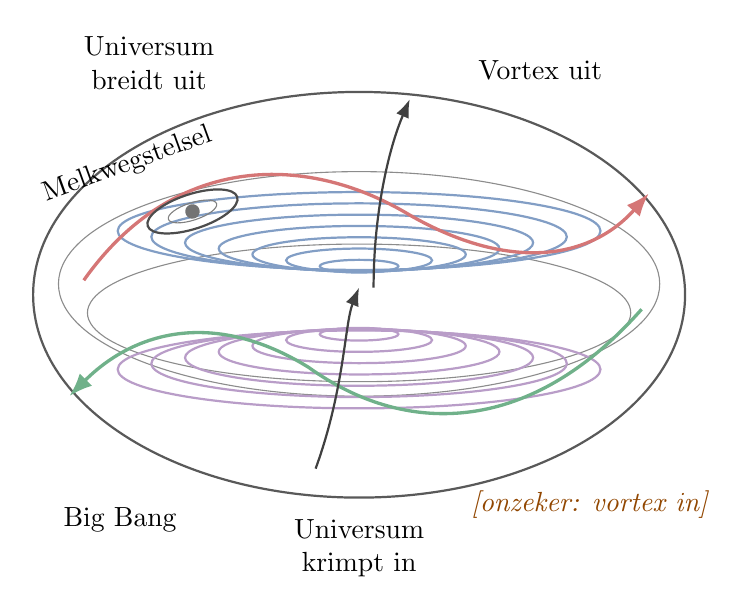
\begin{tikzpicture}[>=Latex,x=1cm,y=1cm,scale=0.92]
  % buitenvorm
  \draw[black!65,thick]
    (0,0) ellipse (4.5 and 2.8);
  \draw[black!45]
    (0,0.15) ellipse (4.15 and 1.55);
  \draw[black!45]
    (0,-0.25) ellipse (3.75 and 0.95);

  % bovenste en onderste vortex
  \foreach \r in {0.35,0.65,...,2.15}
    \draw[inkblue!55,thick]
      (0,{0.30+0.27*\r}) ellipse ({1.55*\r} and {0.25*\r});
  \foreach \r in {0.35,0.65,...,2.15}
    \draw[inkpurple!50,thick]
      (0,{-0.45-0.27*\r}) ellipse ({1.55*\r} and {0.25*\r});

  % spiraalbanen
  \draw[inkred!65,very thick,->]
    (-3.8,0.2) .. controls (-2.6,1.9) and (-0.8,2.0) ..
    (0.7,1.1) .. controls (2.1,0.3) and (3.2,0.5) .. (4.0,1.4);
  \draw[inkgreen!65,very thick,->]
    (3.9,-0.2) .. controls (2.4,-1.9) and (0.7,-2.0) ..
    (-0.7,-1.0) .. controls (-2.0,-0.2) and (-3.1,-0.5) .. (-4.0,-1.4);
  \draw[black!75,thick,->]
    (-0.6,-2.4) .. controls (-0.2,-1.3) and (-0.2,-0.4) .. (0,0.1);
  \draw[black!75,thick,->]
    (0.2,0.1) .. controls (0.2,1.1) and (0.4,2.0) .. (0.7,2.7);

  % melkweg
  \begin{scope}[shift={(-2.3,1.15)},rotate=18]
    \draw[black!70,thick] (0,0) ellipse (0.65 and 0.24);
    \draw[black!50] (0,0) ellipse (0.35 and 0.12);
    \fill[black!55] (0,0) circle (0.10);
  \end{scope}

  % labels
  \node[align=center] at (-2.9,3.2) {Universum\\breidt uit};
  \node at (2.5,3.1) {Vortex uit};
  \node[rotate=20] at (-3.2,1.8) {Melkwegstelsel};
  \node at (-3.3,-3.1) {Big Bang};
  \node[align=center] at (0,-3.5) {Universum\\krimpt in};
  \node at (3.2,-2.9) {\uncertain{vortex in}};
\end{tikzpicture}
\end{center}

\newpage
\subsection*{Rechter notitiepagina: trechter, donut en dodecaëder}

De drie getekende vormen zijn gelabeld als ``Vuvuzela'', ``donut'' en
``dodecahedron''. Tussen de eerste twee staat een plusteken; pijlen verbinden
de vormen met de grote vortexschets op de linker bladzijde.

\begin{center}
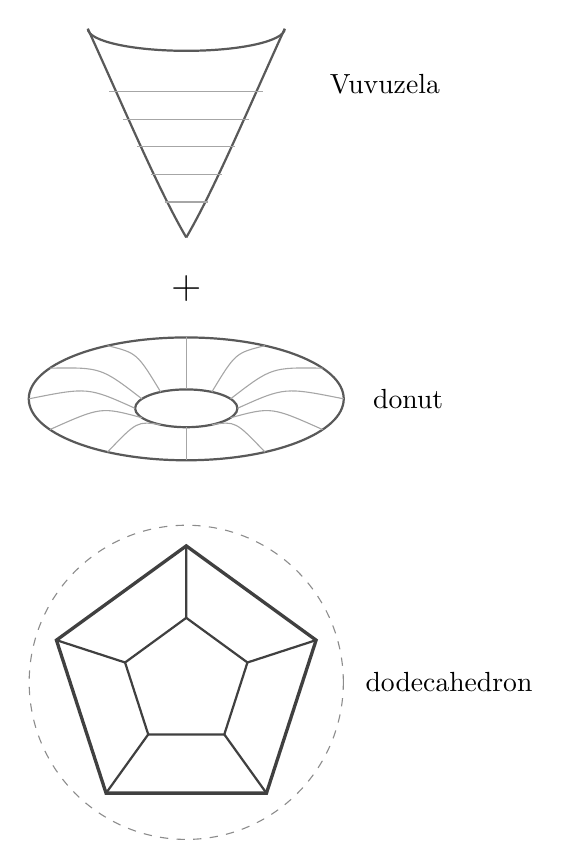
\begin{tikzpicture}[>=Latex,x=1cm,y=1cm,scale=1.0]
  % vuvuzela/trechter
  \draw[black!65,thick] (-1.25,3.3) arc (180:360:1.25 and 0.28);
  \draw[black!65,thick] (-1.25,3.3) .. controls (-0.75,2.2) and
    (-0.35,1.25) .. (0,0.65);
  \draw[black!65,thick] (1.25,3.3) .. controls (0.75,2.2) and
    (0.35,1.25) .. (0,0.65);
  \foreach \y in {1.1,1.45,1.8,2.15,2.5}
    \draw[black!35] ({-0.5*(\y-0.55)},\y)--({0.5*(\y-0.55)},\y);
  \node[anchor=west] at (1.7,2.6) {Vuvuzela};

  \node at (0,0.0) {\Large $+$};

  % torus
  \begin{scope}[shift={(0,-1.4)}]
    \draw[black!65,thick] (0,0) ellipse (2.0 and 0.78);
    \draw[black!65,thick] (0,-0.12) ellipse (0.65 and 0.24);
    \foreach \a in {0,30,...,330}
      \draw[black!35]
        ({0.65*cos(\a)},{-0.12+0.24*sin(\a)}) ..
        controls ({1.25*cos(\a)},{0.15+0.50*sin(\a)}) ..
        ({2.0*cos(\a)},{0.78*sin(\a)});
    \node[anchor=west] at (2.25,0) {donut};
  \end{scope}

  % dodecahedron approximation
  \begin{scope}[shift={(0,-5.0)},scale=1.05]
    \coordinate (A) at (0,1.65);
    \coordinate (B) at (1.57,0.51);
    \coordinate (C) at (0.97,-1.34);
    \coordinate (D) at (-0.97,-1.34);
    \coordinate (E) at (-1.57,0.51);
    \draw[black!75,very thick] (A)--(B)--(C)--(D)--(E)--cycle;
    \coordinate (a) at (0,0.78);
    \coordinate (b) at (0.74,0.24);
    \coordinate (c) at (0.46,-0.63);
    \coordinate (d) at (-0.46,-0.63);
    \coordinate (e) at (-0.74,0.24);
    \draw[black!75,thick] (a)--(b)--(c)--(d)--(e)--cycle;
    \draw[black!75,thick] (A)--(a) (B)--(b) (C)--(c) (D)--(d) (E)--(e);
    \draw[black!45,dashed] (0,0) circle (1.9);
    \node[anchor=west] at (2.05,0) {dodecahedron};
  \end{scope}
\end{tikzpicture}
\end{center}

% --------------------------------------------------------------------------
\newpage
\section*{PDF-pagina 17 --- atomen, lading en tijdruimte}

\subsection*{Linker notitiepagina: waarom atomen aan elkaar plakken}

De tekst bovenaan luidt:

\literalnote{%
In een atoom is er voor elke proton een elektron.}

Daarna volgt de vraag:

\literalnote{%
Waarom plakken atomen aan elkaar?}

De chemische vergelijking is in de scan geschreven als:
\[
2\mathrm{H}^{+}+\mathrm{O}^{2-}=\mathrm{H}_{2}\mathrm{O}.
\]

De toelichting luidt zo letterlijk mogelijk:

\literalnote{%
Wanneer je waterstof een extra lading geeft: $+1$ elektron, en van zuurstof
$2$ ladingen weghaalt, zullen de instabiele atomen elkaar niet afstoten omdat
ze elkaar aanvullen.}

\noindent
De woorden ``ladingen weghaalt'' en de weergegeven ionladingen zijn behouden,
ook al is de formulering chemisch niet volledig consistent.

\newpage
\subsection*{Rechter notitiepagina: massa als roterende lading}

De kop luidt:
\[
\text{``Massa is roterende lading''}.
\]

De schets toont een proton in een vervormd tijdruimterooster, een rode
rotatiepijl en meerdere golvende lijnen.

\begin{center}
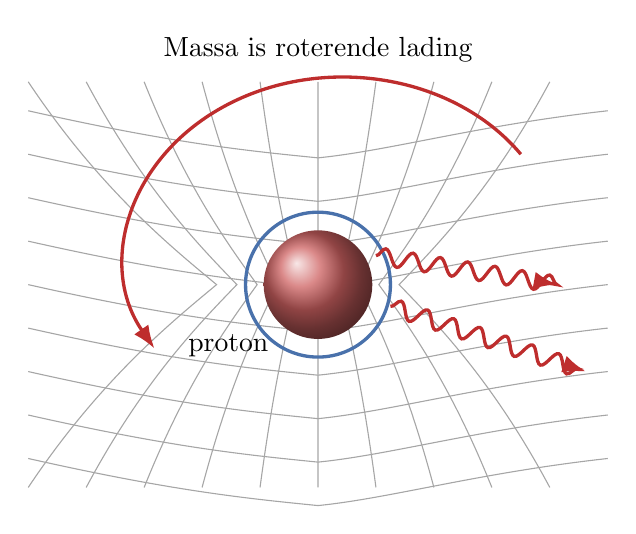
\begin{tikzpicture}[>=Latex,x=1cm,y=1cm,scale=0.92]
  % gekromd rooster
  \foreach \y in {-2.4,-1.8,...,2.4}
    \draw[black!35]
      (-4,\y) .. controls (-2.0,{\y-0.45}) and (-1.0,{\y-0.55}) ..
      (0,{\y-0.65}) .. controls (1.0,{\y-0.55}) and (2.2,{\y-0.2}) ..
      (4,\y);
  \foreach \x in {-4,-3.2,...,4}
    \draw[black!35]
      (\x,-2.8) .. controls ({0.75*\x},-1.3) and ({0.50*\x},-0.5) ..
      ({0.35*\x},0) .. controls ({0.50*\x},0.5) and ({0.75*\x},1.3) ..
      (\x,2.8);

  % centrale lading
  \shade[ball color=inkred!75] (0,0) circle (0.75);
  \draw[inkblue!80,very thick] (0,0) circle (1.0);
  \node[below left] at (-0.55,-0.55) {proton};

  % rotatiepijl
  \draw[inkred,very thick,->]
    (2.8,1.8) arc (35:210:3.0 and 2.5);

  % golven
  \draw[inkred,decorate,decoration={snake,amplitude=3pt,segment length=10pt},
        very thick,->] (1.0,-0.3)--(3.7,-1.2);
  \draw[inkred,decorate,decoration={snake,amplitude=3pt,segment length=10pt},
        very thick,->] (0.8,0.4)--(3.3,0.0);

  \node at (0,3.25) {Massa is roterende lading};
\end{tikzpicture}
\end{center}

Naast en onder de tekening staat:

\literalnote{%
Proton in tijdruimte. Fotonen gaan door tijdruimte op zoek naar een
elektronengolf. Bij de botsing ontstaat er een roterende lading en dus een
massa die naar de kern wordt getrokken.}

% --------------------------------------------------------------------------
\newpage
\section*{PDF-pagina 18 --- waterstof- en zuurstofmodellen}

\subsection*{Linker notitiepagina: waterstof}

Bovenaan staat ``Waterstof atoom --- Hydrogen''. De vermelde samenstelling is:
\[
1\ \text{proton},
\qquad
1\ \text{elektron}.
\]

\begin{center}
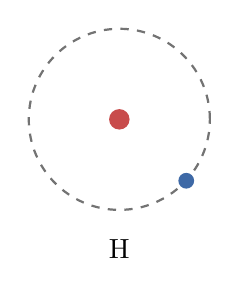
\begin{tikzpicture}[x=1cm,y=1cm]
  \draw[black!55,dashed,thick] (0,0) circle (1.15);
  \proton{0}{0}
  \electron{0.85}{-0.78}
  \node[below=1.4cm] at (0,0) {$\mathrm{H}$};
\end{tikzpicture}
\end{center}

Onderaan staat ``Waterstof Ion $\mathrm{H}^{+}$'', gevolgd door:
\[
1\ \text{proton},
\qquad
2\ \text{elektronen}.
\]

\begin{center}
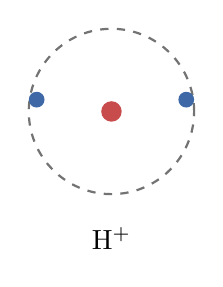
\begin{tikzpicture}[x=1cm,y=1cm]
  \draw[black!55,dashed,thick] (0,0) circle (1.05);
  \proton{0}{0}
  \electron{-0.95}{0.15}
  \electron{0.95}{0.15}
  \node[below=1.35cm] at (0,0) {$\mathrm{H}^{+}$};
\end{tikzpicture}
\end{center}

\literalnote{%
De aanduiding $\mathrm{H}^{+}$ met twee elektronen is letterlijk uit de scan
overgenomen. In de gangbare atoomnotatie zou $\mathrm{H}^{+}$ geen elektron
hebben; een waterstofatoom met twee elektronen wordt als $\mathrm{H}^{-}$
geschreven.}

\newpage
\subsection*{Rechter notitiepagina: zuurstof}

Bovenaan staat ``Zuurstof --- Oxygen''. De vermelde samenstelling is:
\[
8\ \text{protonen},
\qquad
8\ \text{elektronen}\ (2,6).
\]

\begin{center}
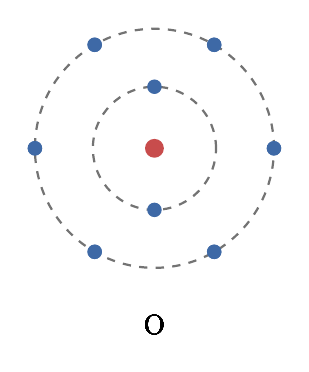
\begin{tikzpicture}[x=1cm,y=1cm,scale=0.92]
  \draw[black!55,dashed,thick] (0,0) circle (0.85);
  \draw[black!55,dashed,thick] (0,0) circle (1.65);
  \proton{0}{0}
  \foreach \a in {90,270}
    \electron{{0.85*cos(\a)}}{{0.85*sin(\a)}}
  \foreach \a in {0,60,...,300}
    \electron{{1.65*cos(\a)}}{{1.65*sin(\a)}}
  \node[below=2.0cm] at (0,0) {$\mathrm{O}$};
\end{tikzpicture}
\end{center}

Daaronder staat ``Zuurstof Ion $\mathrm{O}^{2-}$'', gevolgd door:
\[
8\ \text{protonen},
\qquad
6\ \text{elektronen}.
\]

\begin{center}
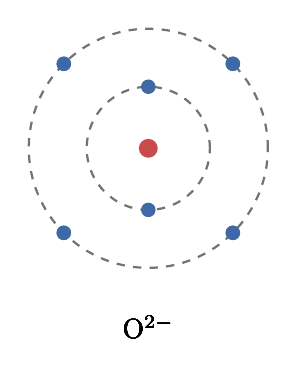
\begin{tikzpicture}[x=1cm,y=1cm,scale=0.92]
  \draw[black!55,dashed,thick] (0,0) circle (0.85);
  \draw[black!55,dashed,thick] (0,0) circle (1.65);
  \proton{0}{0}
  \foreach \a in {90,270}
    \electron{{0.85*cos(\a)}}{{0.85*sin(\a)}}
  \foreach \a in {45,135,225,315}
    \electron{{1.65*cos(\a)}}{{1.65*sin(\a)}}
  \node[below=2.0cm] at (0,0) {$\mathrm{O}^{2-}$};
\end{tikzpicture}
\end{center}

\literalnote{%
Ook deze telling is letterlijk behouden. Gangbaar heeft een neutraal
zuurstofatoom acht elektronen en het ion $\mathrm{O}^{2-}$ tien elektronen.}

% --------------------------------------------------------------------------
\newpage
\section*{PDF-pagina 19 --- Maxwellvergelijkingen en enthalpie}

\subsection*{Linker notitiepagina: veldvergelijkingen}

De vier regels staan in de scan als:

\begin{align*}
\nabla\cdot\mathbf{D} &= \rho,\\
\nabla\cdot\mathbf{B} &= 0,\\
\nabla\cdot\mathbf{E} &= -\frac{\partial\mathbf{B}}{\partial t},\\
\nabla\cdot\mathbf{H} &= \mathbf{J}
  +\frac{\partial\mathbf{D}}{\partial t}.
\end{align*}

\noindent
Bij de laatste twee regels lijkt in het handschrift een punt te staan. In de
gangbare differentiële vorm van de Maxwellvergelijkingen worden daar
rotaties gebruikt:

\begin{align*}
\nabla\times\mathbf{E} &= -\frac{\partial\mathbf{B}}{\partial t},\\
\nabla\times\mathbf{H} &= \mathbf{J}
  +\frac{\partial\mathbf{D}}{\partial t}.
\end{align*}

\newpage
\subsection*{Rechter notitiepagina: enthalpie}

De kop luidt ``Enthalpie $H$ is een grootheid''. De hoofdvergelijking is:
\[
H=U+pV.
\]

De symbolen worden in de scan als volgt toegelicht:

\begin{center}
\begin{tabular}{@{}>{$}l<{$}@{\quad}l@{}}
H & enthalpie in joule,\\
U & inwendige energie in joule,\\
p & druk in pascal, $\mathrm{N\,m^{-2}}$,\\
V & volume, $\mathrm{m^3}$.
\end{tabular}
\end{center}

% --------------------------------------------------------------------------
\newpage
\section*{PDF-pagina 20 --- de Broglie en zwaartekracht}

\subsection*{Linker notitiepagina: Louis de Broglie}

De naam is geschreven als ``Louis de Broglie''. De golflengte staat als:

\begin{align*}
\lambda
  &= \frac{h}{p}
   = \frac{h}{mv}\sqrt{1-\frac{v^2}{c^2}}.
\end{align*}

Daaronder staat het impulsmoment:

\begin{align*}
\mathbf{L}_{\text{impulsmoment}}
  &= \mathbf{R}\times\mathbf{P}_{\text{impulsvector}}.
\end{align*}

De eenheid wordt genoteerd als:
\[
\mathrm{N\,m\,s}.
\]

In SI-basiseenheden is dit gelijk aan:
\[
\mathrm{N\,m\,s}=\mathrm{kg\,m^2\,s^{-1}}.
\]

\newpage
\subsection*{Rechter notitiepagina: zwaartekrachtconstante}

De kop luidt ``Zwaartekracht constante''. De eerste schets toont twee massa's
$m_1$ en $m_2$, op afstand $R$, met tegengesteld gerichte krachten
$\mathbf{F}_1$ en $\mathbf{F}_2$.

\begin{center}
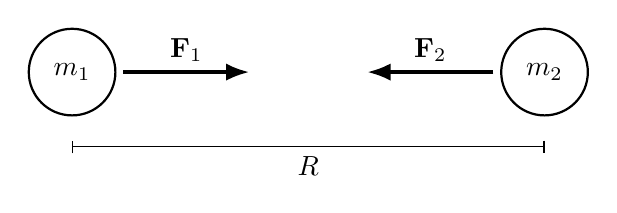
\begin{tikzpicture}[>=Latex,x=1cm,y=1cm]
  \draw[thick] (-3,0) circle (0.55);
  \draw[thick] (3,0) circle (0.55);
  \node at (-3,0) {$m_1$};
  \node at (3,0) {$m_2$};
  \draw[->,very thick] (-2.35,0)--(-0.75,0)
    node[midway,above] {$\mathbf{F}_1$};
  \draw[->,very thick] (2.35,0)--(0.75,0)
    node[midway,above] {$\mathbf{F}_2$};
  \draw[|-|] (-3,-0.95)--(3,-0.95)
    node[midway,below] {$R$};
\end{tikzpicture}
\end{center}

De formule staat als:
\[
F_1=F_2=G\frac{m_1m_2}{R^2}.
\]

Vervolgens wordt een proton--elektronsysteem getekend. Het elektron beweegt
op afstand $r$ of $a_0$ van het proton en er zijn twee tegengestelde
krachtpijlen.

\begin{center}
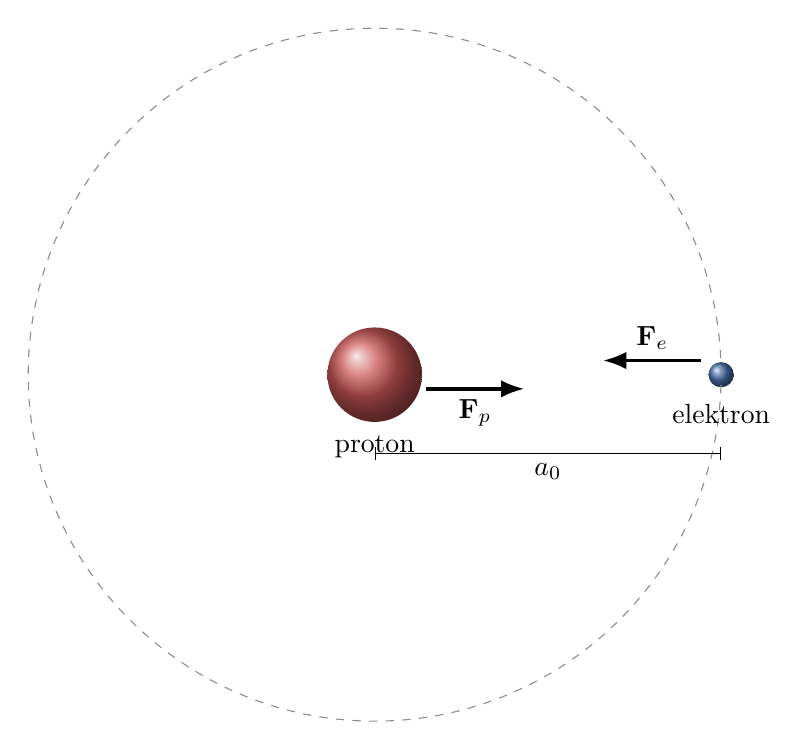
\begin{tikzpicture}[>=Latex,x=1cm,y=1cm]
  \shade[ball color=inkred!80] (-2.2,0) circle (0.60);
  \shade[ball color=inkblue!80] (2.2,0) circle (0.16);
  \draw[black!45,dashed] (-2.2,0) circle (4.4);
  \draw[->,very thick] (1.95,0.18)--(0.7,0.18)
    node[midway,above] {$\mathbf{F}_e$};
  \draw[->,very thick] (-1.55,-0.18)--(-0.3,-0.18)
    node[midway,below] {$\mathbf{F}_p$};
  \draw[|-|] (-2.2,-1.0)--(2.2,-1.0)
    node[midway,below] {$a_0$};
  \node[below] at (-2.2,-0.65) {proton};
  \node[below] at (2.2,-0.25) {elektron};
\end{tikzpicture}
\end{center}

De bijbehorende formule is:
\[
F=G\frac{m_pm_e}{r^2}.
\]

Onderaan staat een moeilijk leesbare numerieke uitwerking. Zo letterlijk
mogelijk gelezen is deze:

\[
\uncertain{1{,}09154928}\times10^{-57}\,\mathrm{N}
=
6{,}67384\times10^{-11}
\frac{m_pm_e}{a_0}.
\]

\noindent
In de laatste breuk lijkt de scan $a_0$ zonder kwadraat te tonen, hoewel
erboven $r^2$ staat. Onder het eerste getal staat met een pijl:
``Proton dat geëxciteerd wordt''.

\end{document}
